\section{Evaluation}

\subsection{Test set and metrics}
The data was split 70/15/15 into training, validation and test sets with a fixed random seed. All hyperparameters were chosen on the validation set. The test set (10,307 rows) was used only once, to produce the numbers in this section, so it shows how the final models perform on data they have not seen.

Our main task is regression: predicting the DC power of the plant. We report three regression metrics:
\begin{itemize}
    \item \textbf{MAE} (mean absolute error): the average size of the error, in the same unit as the power. It is easy to read and explain.
    \item \textbf{RMSE} (root mean squared error): like MAE, but it punishes large mistakes more. This matters for SunCast, because a few large forecast errors hurt the savings estimate more than many small ones.
    \item \textbf{$R^2$}: the share of the variation in power that the model explains (1 is perfect).
\end{itemize}

The course guide also asks for Precision, Recall, F1 and AUC-ROC, which are classification metrics. We therefore added one binary task: is the output \emph{high} or \emph{low}? A row is labelled high when its DC power is above the median DC power of the training set (440.5~kW). The median comes from the training set only, so no test information is used. Because the threshold is a median, the two classes are about the same size, so accuracy alone would not be misleading here. We still report Precision, Recall, F1 and AUC-ROC because they show separately how many low-output hours are wrongly called high (Precision), how many high-output hours are missed (Recall), and how well the predicted power ranks high rows above low rows (AUC-ROC). For the app this matters: calling a low-output hour high makes the savings look better than they are, while missing a high-output hour hides real savings.

\subsection{Test results}
Table~\ref{tab:testreg} shows the regression results and Table~\ref{tab:testclf} shows the results for the high versus low task.

\begin{table}[H]
\centering
\begin{tabular}{lrrr}
\toprule
\textbf{Model} & \textbf{MAE} & \textbf{RMSE} & \textbf{R\textsuperscript{2}} \\
\midrule
Physics baseline (sunlight only) & 234.89 & 503.25 & 0.9844 \\
Physics baseline (sunlight + temperature) & 208.32 & 466.90 & 0.9866 \\
Neural network & 178.26 & 417.49 & 0.9892 \\
Gradient boosting & 153.59 & 369.18 & 0.9916 \\
\bottomrule
\end{tabular}
\caption{Regression metrics on the test set (10,307 rows), including the two physics baselines.}
\label{tab:testreg}
\end{table}

\begin{table}[H]
\centering
\begin{tabular}{lrrrr}
\toprule
\textbf{Model} & \textbf{Precision} & \textbf{Recall} & \textbf{F1} & \textbf{AUC-ROC} \\
\midrule
Gradient boosting & 0.9973 & 0.9975 & 0.9974 & 1.0000 \\
Neural network & 0.9981 & 0.9959 & 0.9970 & 1.0000 \\
\bottomrule
\end{tabular}
\caption{Metrics for the high versus low output task on the test set (threshold 440.5~kW).}
\label{tab:testclf}
\end{table}

Gradient boosting is the better model on every regression metric. Its MAE is about 14\% lower and its RMSE about 12\% lower than those of the neural network, and its $R^2$ is slightly higher. Its test MAE (153.59) is close to its validation MAE (151.82), and the neural network behaves the same way (178.26 on test, 174.37 on validation), so we see no sign that the settings were over-fitted to the validation set. The mean DC power of the test rows is about 3,155, so the average error is about 4.9\% of it for gradient boosting and about 5.6\% for the neural network. On this evidence we treat gradient boosting as our main model and the neural network as the comparison.

Both models separate high from low output almost perfectly (F1 about 0.997, AUC-ROC 1.00). The differences between them on these metrics are tiny (0.0004 in F1) and should not be read as one model being better. This task is easy: the output is exactly zero at night, and during the day most rows are far above the threshold, so only the rows near sunrise and sunset are close to it. An AUC-ROC of 1.00 therefore does not mean that the models are perfect. The regression metrics and the error analysis in the next section say much more about their quality.

\begin{figure}[H]
\centering
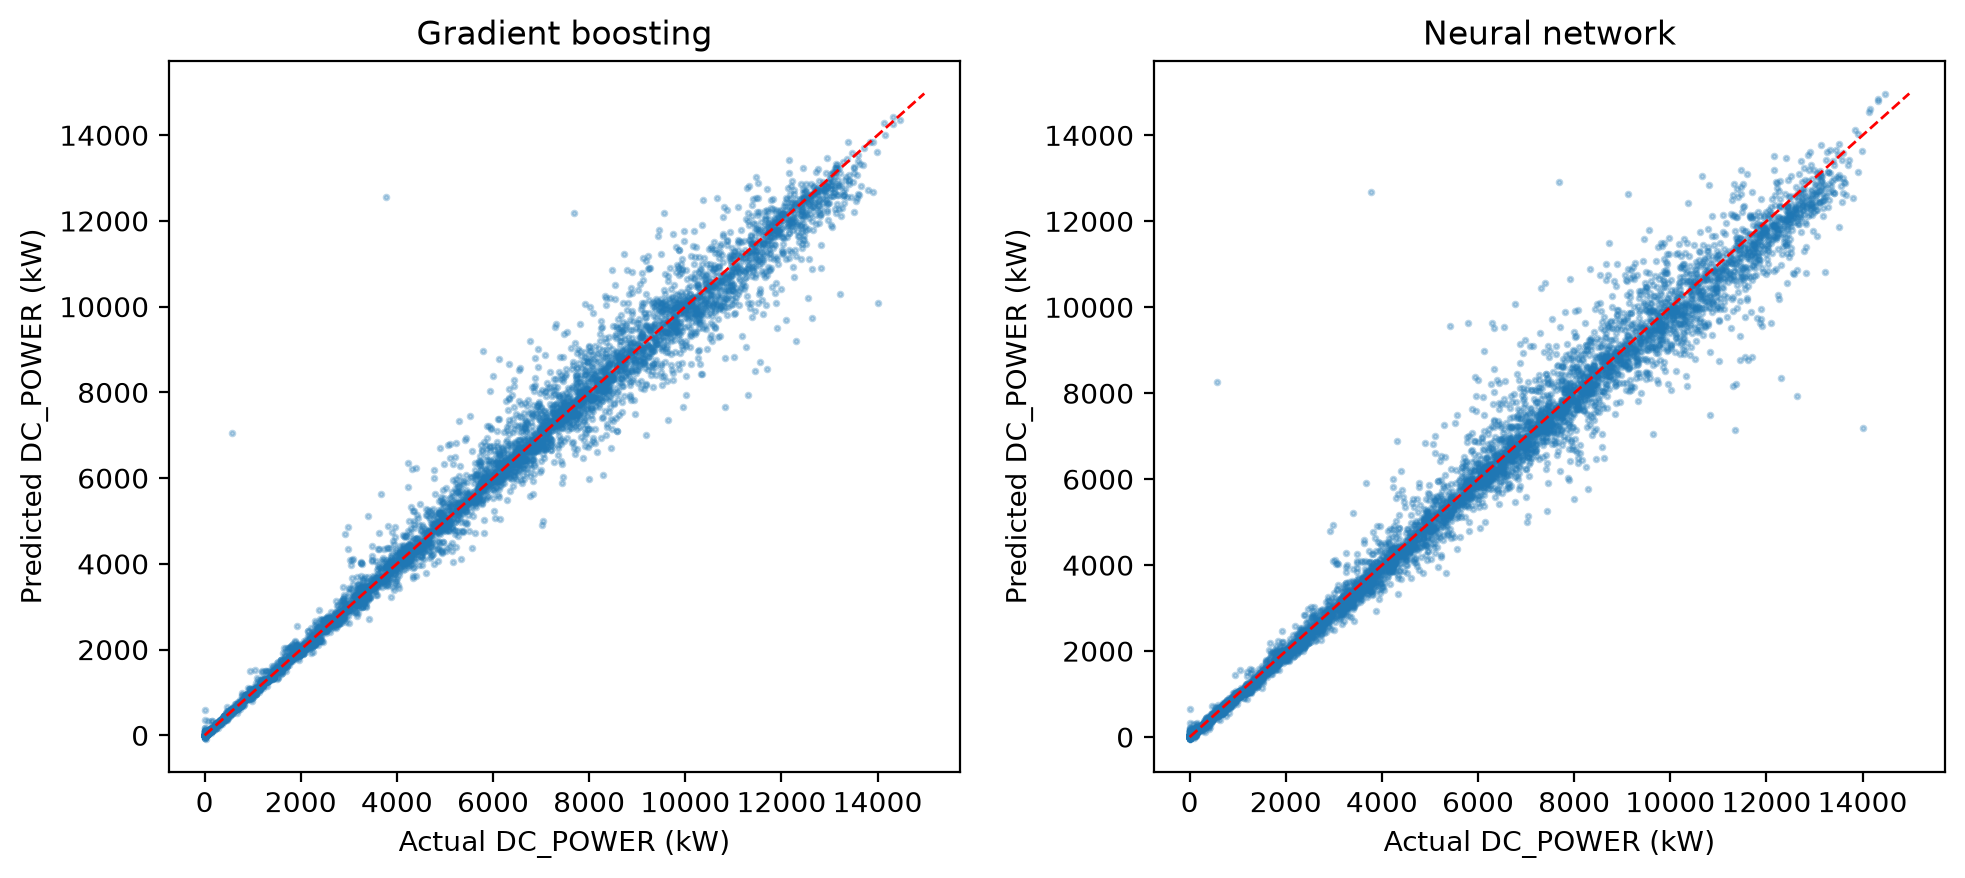
\includegraphics[width=\textwidth]{predicted_vs_actual.png}
\caption{Predicted against actual DC power on the test set for both models. Points on the diagonal line are perfect predictions.}
\label{fig:predactual}
\end{figure}